\begin{frame}[fragile]{Schema del database Sakila}
\begin{figure}
    \centering
        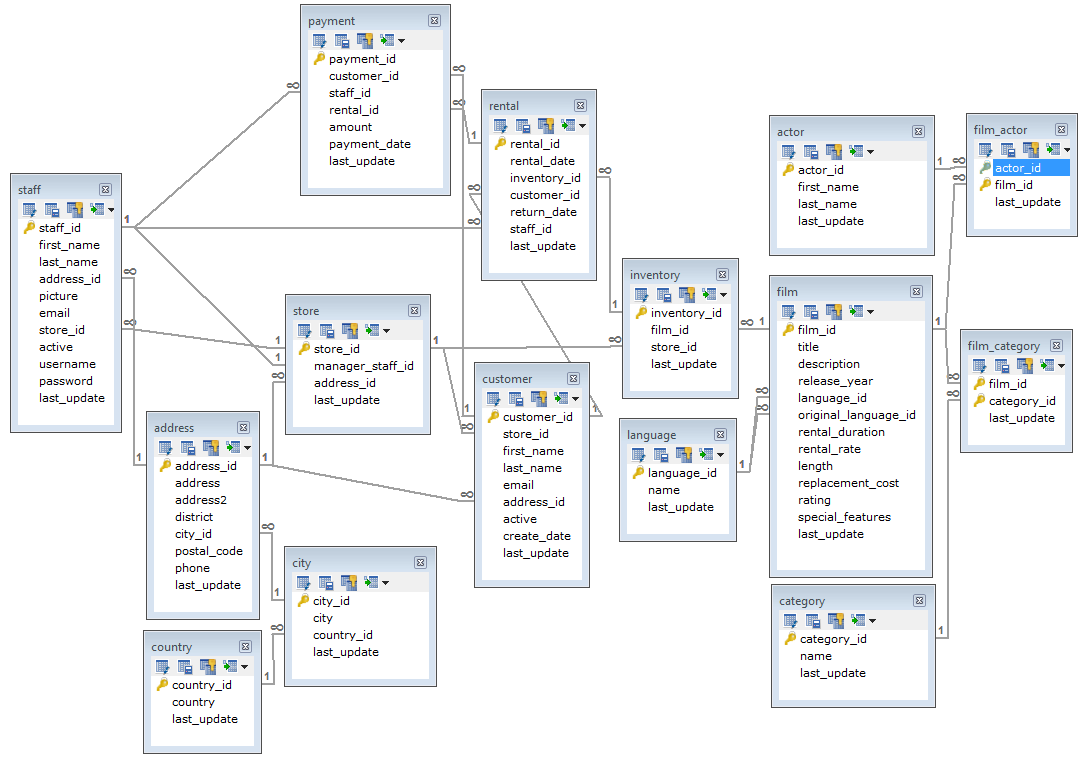
\includegraphics[width=.65\textwidth]{img/db-sakila.png}
    \end{figure}
\end{frame}
%
\begin{frame}[fragile]{Sakila: Es. 1}
Quali attori hanno il nome `Scarlett'?
\pause
\begin{lstlisting}
SELECT *
FROM actor
WHERE first_name = `Scarlett';
\end{lstlisting}
\end{frame}
%
\begin{frame}[fragile]{Sakila: Es. 2}
Quali attori hanno il cognome `Johansson'?
\pause
\begin{lstlisting}
SELECT *
FROM actor
WHERE last_name LIKE `Johansson';
\end{lstlisting}
\pause
oppure
\begin{lstlisting}
SELECT *
FROM actor
WHERE last_name = `Johansson';
\end{lstlisting}
\end{frame}
%
\begin{frame}[fragile]{Sakila: Es. 3}
Quanti cognomi distinti di attori ci sono?
\pause
\begin{lstlisting}
SELECT COUNT(distinct last_name)
FROM actor;
\end{lstlisting}
\end{frame}
%
\begin{frame}[fragile]{Sakila: Es. 4}
Quali cognomi non si ripetono?
\pause
\begin{lstlisting}
SELECT last_name
FROM actor
GROUP BY last_name
HAVING COUNT(*) = 1;
\end{lstlisting}
\end{frame}
%
\begin{frame}[fragile]{Sakila: Es. 5}
Quali cognomi compaiono pi\`u di una volta?
\pause
\begin{lstlisting}
SELECT last_name
FROM actor
GROUP BY last_name
HAVING COUNT(*) > 1;
\end{lstlisting}
\end{frame}
%
\begin{frame}[fragile]{Sakila: Es. 6}
Qual \`e l'attore che ha recitato nel maggior numero di film?
\pause
\begin{lstlisting}
SELECT actor.actor_id, actor.first_name, actor.last_name,
COUNT(actor.actor_id) AS film_count
FROM actor JOIN film_actor
GROUP BY actor_id
ORDER BY film_count DESC
LIMIT 1;
\end{lstlisting}
\end{frame}
%
\begin{frame}[fragile]{Sakila: Es. 7}
Inserire un record per rappresentare `Mary Smith' che oggi affitta `Academy Dinosaur' da `Mike Hillyer' presso lo Store 1.
\pause
\begin{lstlisting}
INSERT INTO rental
(rental_date, inventory_id, customer_id, staff_id)
VALUES
(NOW(), 1, 1, 1);
\end{lstlisting}
\end{frame}
%
\begin{frame}[fragile]{Sakila: Es. 8}
Qual \`e la lunghezza media di tutti i film del DB sakila?
\pause
\begin{lstlisting}
SELECT AVG(length)
FROM film;
\end{lstlisting}
\end{frame}
%
\begin{frame}[fragile]{Sakila: Es. 9}
Qual \`e la durata media dei film per categoria?
\pause
\begin{lstlisting}
SELECT category.name, AVG(length)
FROM film JOIN film_category
JOIN category
GROUP BY category.name
ORDER BY AVG(length) DESC;
\end{lstlisting}
\end{frame}
%
\begin{frame}[fragile]{Sakila: Es. 10}
Elenco i titoli di tutti i film che durano pi\`u di 113 minuti:
\pause
\begin{lstlisting}
SELECT title
FROM film
WHERE length >= 113;
\end{lstlisting}
\end{frame}
%
\begin{frame}[fragile]{Sakila: Es. 11}
Elencare i film la cui durata \`e compresa tra 130 e 150 minuti (estremi compresi) e il cui rating \`e NC-17:
\pause
\begin{lstlisting}
SELECT title
FROM film
WHERE length >=130 AND length <= 150 AND rating = `NC-17';
\end{lstlisting}
\pause
oppure
\begin{lstlisting}
SELECT title
FROM film
WHERE length BETWEEN 130 AND 150 AND rating = `NC-17';
\end{lstlisting}
\end{frame}
%
\begin{frame}[fragile]{Sakila: Es. 12}
Elencare nome e cognome di tutti gli attori che hanno recitato nel film ``TEEN APOLLO''.
\pause
\begin{lstlisting}
SELECT first_name, last_name FROM film, actor, film_actor
WHERE film.film_id = film_actor.film_id
AND actor.actor_id = film_actor.actor_id
AND film.title = `TEEN APOLLO';
\end{lstlisting}
\pause
oppure
\begin{lstlisting}
SELECT first_name, last_name
FROM film JOIN film_actor ON film.film_id = film_actor.film_id
JOIN actor ON actor.actor_id = film_actor.actor_id
AND film.title = `TEEN APOLLO';
\end{lstlisting}
\end{frame}
%
\begin{frame}[fragile]{Sakila: Es. 13}
\vspace{.5cm}
Indicare il numero di film e la durata media dei film in cui ha recitato ZERO CAGE.
\pause
\begin{lstlisting}
SELECT COUNT(*) AS `n. film' , AVG(length) AS `durata media'
FROM film JOIN film_actor
ON film.film_id = film_actor.film_id 
JOIN actor ON actor.actor_id = film_actor.actor_id
WHERE actor.first_name = `ZERO' AND actor.last_name=`CAGE';
\end{lstlisting}
\end{frame}
%
\begin{frame}[fragile]{Sakila: Es. 14}
Elencare gli attori per nome, cognome e numero di film fatti, ordinati da chi ha fatto pi\`u film a chi ne ha fatti meno e in caso di ugual numero di film ordinarli per cognome.

Nell'elenco devono comparire solo gli attori che hanno fatto pi\`u di 33 film (33 compreso).
\pause
\begin{lstlisting}
SELECT first_name, last_name, count(*) AS `n. film'
FROM film JOIN film_actor
ON film.film_id = film_actor.film_id 
JOIN actor ON actor.actor_id = film_actor.actor_id
GROUP BY actor.actor_id
HAVING numero_film >= 33
ORDER BY numero_film DESC, last_name;
\end{lstlisting}
\end{frame}
%
\begin{frame}[fragile]{Sakila: Es. 15}
Trovare il film con la durata maggiore, indicandone titolo e durata.

Se fossero pi\`u di uno, elencarli in ordine di titolo.
\pause
\begin{lstlisting}
SELECT title, length
FROM film
WHERE length = (
    SELECT MAX(length)
    FROM film
    )
ORDER BY title;
\end{lstlisting}
\end{frame}
%
\begin{frame}[fragile]{Sakila: Es. 16}
Trovare quanti sono i film la cui durata \`e maggiore di almeno 60 minuti della durata media di tutti i film.
\pause
\begin{lstlisting}
SELECT COUNT(*) AS `n. film'
FROM film
WHERE length > (
    SELECT AVG(length) + 60
    FROM film
);
\end{lstlisting}
\end{frame}
%